\begin{figure}[htbp]
\centering
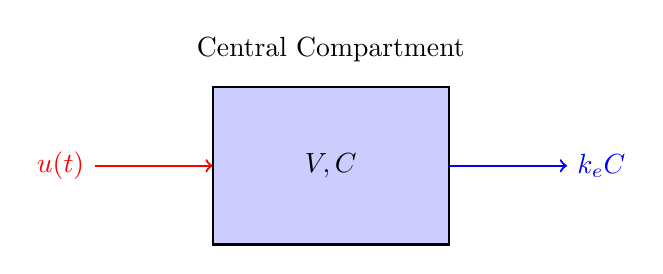
\begin{tikzpicture}
    % Compartment
    \draw[thick, fill=blue!20] (0,0) rectangle (3,2);
    \node at (1.5,1) {$V, C$};

    % Input (infusion)
    \draw[->, thick, red] (-1.5,1) -- (0,1) node[left, pos=0] {$u(t)$};

    % Elimination
    \draw[->, thick, blue] (3,1) -- (4.5,1) node[right] {$k_e C$};

    % Labels
    \node[above] at (1.5,2.2) {Central Compartment};
\end{tikzpicture}
\caption{One-compartment pharmacokinetic model.}
\label{fig:one_compartment}
\end{figure}
